{\fontsize{12}{14}\selectfont 

\begin{figure}[H]
  \centering
  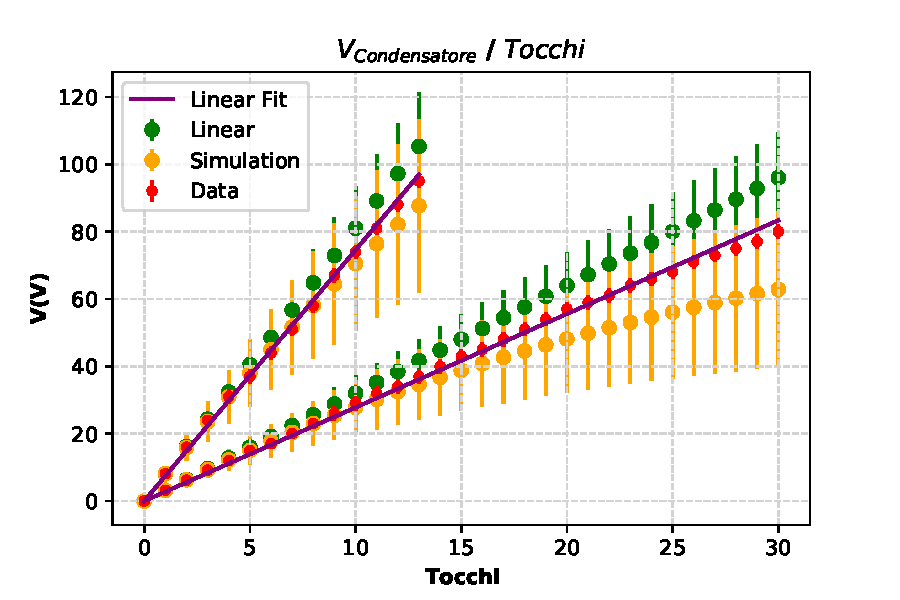
\includegraphics[width=13cm]{Figures/Grafico_Parte2.pdf}
  \caption{Grafico della tensione (in V) in funzione del numero di tocchi per due set differenti. L'errore sulla tensione è pari all'$1\%$ del f.s. + $1$ digit. Le simulazioni si avvicinano all'andamento del rispettivo set di dati ma non lo descrivono esattamente. Il fit è nella forma $V = \text{pendenza} \cdot \text{tocchi}$, quindi passante per lo 0. Nel fit lineare si nota come gli ultimi punti si trovano al di sotto della retta mentre i primi al di sopra di essa, evidenziando come la carica trasferita diminuisca ad ogni tocco.}
  \label{fig:GraficoParteII}
\end{figure}

\begin{figure}[H]
  \centering
  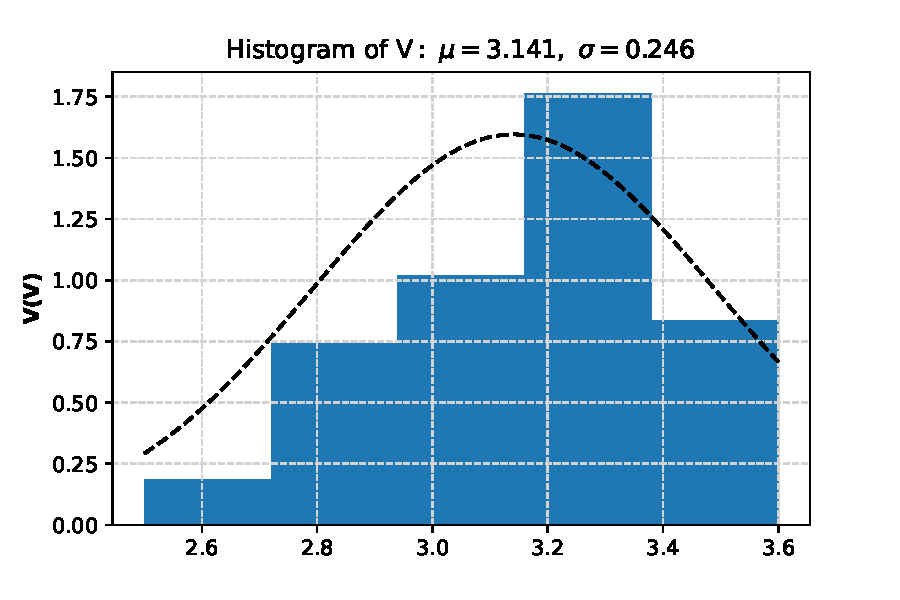
\includegraphics[width=11cm]{Figures/Grafico_Parte2_Carica_Trasferita.pdf}
  \caption{Istogramma della tensione (in V) ai capi del condensatore dopo un tocco, con la sfera carica a $1 kV$. Ci si aspetta una distribuzione gaussiana dei dati che tramite un fit risulta caratterizzata da $\mu = 3.141 V$ e $\sigma = 0.246 V$.}
  \label{fig:GraficoParteIICarica}
\end{figure}

La carica trasferita con il suo errore statistico (ottenuto propagando in quadratura gli errori) è risultata essere:

\begin{equation*}
    Q = \left(C_{sistema} + \dfrac{\varepsilon \cdot A}{d}\right) \cdot V = (4.7 \pm 0.5)\cdot 10^{-10} C
\end{equation*}



\par}